\section{Software development method}
\subsection{What is Agile?}

Agile is a methodology for software developement. It is iterative which means it is based on tide cycles. Those cycles start with the requirements of what is going to be done during that period of time.
It is followed by the analysis, design and coding. After that comes the testing and it ends with the evaluation of the cycle.
It favors quick meetings and short documentations over huge requirements that are frozen at the beginning of the projet coupled with a huge documentation.
Agile is based on time and not on features. We have a certain periode of time to try to at least do a certain number of features. If there is some time left , we can keep going and implements another one.
Is is also very colaborative and for the most part requiers the whole team to work together.

\todo[inline]{Cette partie ne doit pas faire une explication façon
    Wikipédia ; Pourquoi une méthodologie ? Laquelle utilisons-nous ?
    Pourquoi ? Comment organisation le travail (rôles, respect des
consignes, deadlines) ?}

\subsubsection{Why use agile for this project?}

This project has features in different categories (Must have,Should have,Could have,Would like to have). If we used a non agile methodology, we would have to chose at the very begining all the features that we want to implement.
It is not an optimal solution for an university project since we have some other work to do. It is very hard at the begining of the semester to know how much we will be able to implement. This is why it is interresting to use a methodology that favorise change like Agile.
We are also used to code in a Agile way since we started having project. In team project we would always code with different poeple working on the same project to exchange idea or coordonate in an easier way.
We have weekly meetings with the project leader which fits well for Agile since we have to deliver something every week.
To conclude, there might be some more busy weeks because of other classes assignments and an agile methodology will allow us to be more flexible on the features we will implement during a periode.

\subsubsection{Development methodology}
Scrum is an agile methodology to manage a project and is usually used to manage software development. It's more of a framework for managing process than a real methodology.\newline

The main idea behind scrum and behind agile methodology in general is not to provide a full detailed description of how everything has to be done. It leaves it to the scrum software development team who will know best how to solve those problems. We speak about the desired outcome not the implementation details.\newline

There is two mains roles in Scrum. The ScrumMaster, a coach really, helping the team members to use the scrum process to perform at the highest level. And the Product Owner (PO) who is the customers or users and guides the team toward building the right product. In our case it is the ASBL.\newline

Scrum works with a backlog containing the list of all the functionality. This list is ordered and the team always works on the most valuable features first. This backlog is created at the start of the project. It's usually composed of user stories which is a short descriptions of functionality described from the perspective of a user or a customer.\newline

Scrum works with sprints. It's a short period of item from one to four week long (usually two weeks) where the team works and provide a potentially shippable product at the end of it. There is a planning meeting at the start of each sprint. During the meeting the team decide how many items they can commit to. The sprint backlog is then created. All those features will be done, coded, tested and integrated with the evolving product. At the end of each sprint, the team show to the PO their work and he can provide feedback that could influence the next sprint. This may lead to add, remove or revise items in the product backlog.\newline

We decide to choose \enquote{Agile} and Scrum as a development method because
everyone in the team worked at least once with this method (in the 4th
project of computer science bachelor) and it fits perfectly with this
kind of project with 8 team members.\newline

\iffalse
\subsubsection{Back End development}
The back end handles everything related to the web server and the database. Using a framework will allow us to focus on the website development without worrying too much about security,use management, administration panel, etc.\newline

We are going to use \textbf{Django}, an open-source framework, for the back-end. It has a large community and is easy to learn. Some group members already have experience with this framework which is gonna make it easier for everybody to get started quickly.\newline

Another advantage of \textbf{Django} is the database management. \textbf{Django} uses Django-ORM which makes it really easy to communicate with the database. Django-ORM writes the SQL statements by itself. This allows us to use any type of database(sqllite,mySQL,PostgreSQL) and change it during the project development without impacting the rest of the project.
\textbf{Django} uses python as programming language. Python is easy to learn and we have to learn it for our Artificial Intelligence class.
Python is also very clean and easy to read thanks to it's indentation syntax. Once again, multiple team members had experience with python which is good to get started faster.\newline

We also looked at the possibility of doing our website with PHP. Beside the fact that PHP is getting old, it is still the most used back-end language on the web. It historical security problems and the fact that the code is included inside the HTML are two main reasons why we didn't chose PHP.\newline

Ruby seems like a pretty good option as well and looked a lot like python but none of our team members had experience with it. JavaScript was another option but the only framework that some team member knew with JavaScript is \textbf{NodeJS} which was used in a previous project. Most people didn't have a good experience with it(setting up the project may be long and there are a lot of differents middle wares to install to make your project running).

\subsubsection{Front-End development}

There are lots of tool to build the website design. The three main tools are HTML (creating the web site elements), CSS (customize elements with color, placement and more) and JavaScript (used for validation, animation, forms, etc). Like the back end, there are frameworks build around those tools making the design building easier, better and faster. We will mainly use \textbf{Bootstrap}. It's a framework using HTML, CSS and JavaScript for developing responsive website for desktop and mobile. \textbf{Bootstrap} alone isn't enough to build the whole website design. An other framework we are planning to use is \textbf{Angular JS}. It extends HTML with new attributes to handle events, forms, input, validation and more. With those two framework we'll be able to build to most part of the application. We'll just need to add some more CSS to customize it.

\subsubsection{Management}

We are using \textbf{Git} to have a repository for our codes and reports or the project. We'll also use \textbf{Trello}, a free web-based project management application using kanban paradigm. Both \textbf{Git} and \textbf{Trello} were used in the project 4 last year and we all are familiar with these tools.

We will use Trello as a kanban and GitHub as a host for the code. \newline
\fi

\section{User stories (requirements)}
Based on the customer desired functions and features, we end up with the
following requirements (Must-have, Should-have, Could-have, Would like
to have):

\section{Requirements}
\label{sec:Requirements}

\todo[inline]{Relire et/ou corriger}

In this second section, we will present the various requirements on which we
based the development of the website. All the requirements were given by the
client in paper format or verbally, and we tried our best to fulfill most of
them. The following section will only develop the more interesting
and more significant ones, as there are too many of them to detail them all.

\subsection{Players registration}
\label{sub:Players registration}

\subsubsection{Player registration form}
\label{subs:Registration form}

\todo[inline]{Relire et/ou corriger}

The first requirement is to allow each participant of the tournaments to
register on the website. This is done through the user registration form,
accessible from the front page of the website in the top-right menu.
In this form, the participant has to fill in all the information needed to
create a new account, such as his or her personal email address or the account
password, but also information about him or herself (at least the ones that
are mandatory in order to be enlisted into a tournament).\newline

Some of these fields are limited by a set of values, such as the gender or the
player's rank. Each field is then automatically verified, to make sure
everything has the correct format, and no mandatory information is missing.\newline

Once everything is checked, an email is sent to the given email address,
including a link to confirm the email address, indispensable to complete
the registration process. It is also important to notice that neither the
registration to a tournament nor the registration of a court will be accessible
until the email address has been confirmed. All the personal information can
be edited later on by the user, through the page of his or her profile edition,
on the top-right menu when logged in. Finally, it is during the registration
process that the geolocalisation is computed, based on the physical address
of the player, allowing us to integrate the eco-friendly requirement requested
by the client. \newline

We have chosen to work with accounts instead of the old registration process.
The advantage of a account-wide access is that everything becomes way easier
to manage the data of the players, and which consequently eases many other
processes such as the management of pairs, groups, and tournaments as a whole.

\subsubsection{Player management}
\label{subs:Player management}

\todo[inline]{Relire et/ou corriger}

After the player's registration, it is necessary to be able to manage all the
registered players on the website. All of it is made possible through the staff
pages of the website, in the user management tab, which is only accessible
to authorized staff members. In this tab, all the registered users on the
website are available for consultation with a single click in a list of users.
The information of a user can be modified if needed by the staff members
themselves. It is also possible to perform a search on one or several fields,
such as the name, address, or the payment status, in order to slim the number
users in the list.

\subsection{Pair registration}
\label{sub:Pair registration}

\subsubsection{Pair registration form}
\label{subs:Pair registration form}

\todo[inline]{Relire et/ou corriger}

Once a player is registered on the website, he has to find a partner in order
to compete in any available tournament. Since each player has only one account
for him or herself, he or she should be able to constitute a pair with another
player of the website. This is done through the pair registration form,
which only accessible for users with a confirmed email address. In this form,
the user can go through all the others players in the system, and select
the one he wants to pair with. To make this process easier, the user also has
the possibility to perform a search on several fields, such as the first or
last name, to find his or her partner. \newline

Once the partner has been selected, the user can select between several extra
services. He also has the opportunity to leave a comment, for wishes and/or
remarks, in a text area at the bottom of the page. When the user sends the
pair registration demand to the partner, several automated checks are performed
to assign the pairs to the correct tournament. These checks are based
on the criteria given by the client for each tournament, that is the age and
gender of the players. \newline

Once the pair is created and correctly assigned to a tournament, a mail
is sent to each player of the pair with a summary of all the information on the
newly created pair.

\subsubsection{Payment methods}
\label{subs:Payment methods}

\todo[inline]{Relire et/ou corriger}

The payment methods are available to a pair after the registration to one
tournament. Each member of the pair can choose to pay for the registration and
extra fees, with several payment methods: MasterCard, Visa, Paypal or credit
transfer. After the payment of the fees, the status of the pair is updated,
with the field \textit{Pair payment validated by the staff} ticked.\newline

The payment methods page is implemented, but the payment methods processes
themselves are not. This is due to requirement of an actual account,
with the confidential information of the client, to be fully functional,
which were of course not given. Thus, we have decided to not implement
the payment process with false accounts, which would have been replaced
by the client anyway. In the end, everything is in place for the automated
payment process to be operational, with the exception of the setup for the
client banking accounts.

\subsubsection{Extra management}
\label{subs:Extra management}

\todo[inline]{Relire et/ou corriger}

Another requirement is the ability to manage extra services by staff members,
which will be suggested to the players during the pair registration form.
This is made possible in the \textit{Extra} tab of the staff portal, in which
new extras can be created, and existing ones can be modified or deleted.
Their name, description and price are displayed and editable,
and the number of players that ordered these extras are visible on the list
of extras, on the right-side of each extra. The date of the next tournament
and the inscription fees are also editable in this tab,
on the upper-most module.

\subsubsection{Pairs management}
\label{subs:Pairs management}

\todo[inline]{Relire et/ou corriger}

Similarly to the player management tab, which allows the staff to interact with
all the registered players on the website, the pair management tab is the page
where all the pairs are accessible to the staff. These pairs are displayed in a
very user-friendly manner, with the information of both players in the
pair, viewable and editable in just one click. The information on pairs are
also editable if needed. \newline

A search module is also present, with the same mechanism as the one described
in the player management tab, with results limited to the ones having partially
matching data. Staff members can also print a given pair in the PDF format,
by simply clicking on the corresponding button.

\subsection{Courts registration}
\label{sub:Courts registration}

\subsubsection{Court registration form}
\label{subs:Court registration form}

\todo[inline]{Relire et/ou corriger}

As soon as a user has a registered account on the website,
he or she has the possibility to register one or multiple tennis courts that
will be used for the tournaments. This can be done through the court
registration form, which is directly accessible from the navigation menu
when the user is logged on the website. Several fields are needed to register
a court, such as the exact address and location of the court, or the
availability of the court. Once all the mandatory fields are filled, several
automated checks are performed to be sure that the information are valid.
The address of the court is also checked with geolocalisation tools.
Once every field is checked and confirmed by the user, the new court is
created and displayed under the court tab of the website. A staff member
has to validate this court in order to be listed as an available court
in the tournaments.

\subsection{Group creation}
\label{sub:Group creation}

\todo[inline]{Relire et/ou corriger}

One of the biggest and more challenging requirement of this project is the
group creation in a tournament. Each tournament has to be composed of
several groups of players, where each players is dispatched according to
his or her rank, age, and even the ecological footprint (that is, the distance
from his or her house to the court to play and to the HQ of ASMAE)
using the geolocalisation. All of it is achieved on the tournament tab, which is
only available to authorized staff members. On this page, all the
groups for each tournament can be automatically generated according to the
previous criteria. The number of groups and the number of players per group
can also be adjusted using the corresponding fields. Once everything is set,
one click on the generate button creates the groups. \newline

After the groups are generated, it is still possible to modify them at will, by
swapping two players of different groups. This can be done by dragging a pair
entry and dropping it on another pair entry, or by clicking on two different
pairs. Each group also has to have a leader and a court to play on.
This is made possible by clicking on the corresponding buttons that
automatically assign them, or they can be picked by hand by using the
corresponding fields. Finally, all the requests and comments made by the
players and the court owners are displayed, giving some indications on how
to efficiently set the pairs, leaders, and courts in the groups for the staff.
\newline

Once everything is set, the groups can be either saved (and modified later on)
or validated, meaning that they can no longer be adjusted. An email is then
sent to all the players in the tournament when groups are validated.

\subsubsection{Group scores}
\label{subs:Group scores}

\todo[inline]{Relire et/ou corriger}

Once the groups have been created, and all the matches of a group have
finished, a staff members can put the scores of each match in the groups
management page of the tournament. There, he or she can put the scores of the
match of a group using an interactive score board. He or she can edit and save
all the scores before validating them for good, so that the staff can gradually
complete the board as the scores comes. Once all the scores are entered and
validated, the total points of each pair is computed, which will then be of
some use in order to select the pairs for the afternoon elimination tournament.
\newline

\subsubsection{Printable version of groups}
\label{subs:Printable version of groups}

\todo[inline]{Relire et/ou corriger}

An important requirement is to be able to print the groups of a given
tournament, with all necessary information, such as the empty scoreboard, the
pairs, and the courts. On the group tab of the staff portal, a staff member can
print one group or all groups of a tournament in the PDF format, containing
all the above information.

\subsection{Knock-off tournaments}
\label{sub:Knock-off tournaments}

\subsubsection{Knock-off tournament creation}
\label{subs:Knock-off tournament creation}

\todo[inline]{Relire et/ou corriger}

After completion of the morning matches, and after all the scores of all groups
have been encoded, the afternoon matches have to be determined.
The authorized staff members can choose which pairs will play
in the afternoon by ticking the corresponding pair entry on the first page
to create the tournament tree. Once all the desired pairs have been picked,
the staff members can order the pairs by hand, using drag-and-dropping,
to decide who's going to face whom in the first rounds of the knockoff table.
If the number of pairs is even, each pair will have an opponent, and all pairs
will play in the first round. On the other hand, if the number of pairs is odd,
then the staff has to decide the pairs that will directly pass
the first round, which could be based on their ranking, or any other criterion.
\newline

After every newly created knock-off tournament, an email will automatically be
sent to the players, which especially contains the information on the pairs and
the court they will be playing on.

\subsubsection{Knock-off tournament management}
\label{subs:Knock-off tournament management}

\todo[inline]{Relire et/ou modifier}

Another requirement is the management of the knock-off tournaments. First of
all, each knock-off tree is printable, including the details of the court.
This is mostly intended to the players, as they can be told on any practical
information, such as where and when they have to play, and against whom.
\newline

Once a match has been played, the score can be entered onto the interactive
tree branches: they are clickable, so staff members just have to select one of
two pairs of a match to input the score of the match. Based on the score
the winners is automatically put in the next step of the tree. Thus, the next
match is immediately visible on the tree; this process goes on until every
match is played and there is a winner of the tournament.

\subsection{Staff management}
\label{sub:Staff management}

\subsubsection{History management}
\label{subs:History management}

\todo[inline]{Relire et/ou modifier}

When several members of the staff are working on the same part of the website,
it can be useful to know who modified a given entity, or what has been modified.
This is implemented on the history tab, accessible by the staff members. On
this page, the date, name of the staff member, section of the website, data
modified and details are displayed. All the staff pages have a short version of
the history log, containing only the most recent changes made in the given
section. For instance, on the bottom of the user management tab, there is a
history log that contains only the last 15 changes that are related to users.

\subsubsection{Permissions management}
\label{subs:Permissions management}

\todo[inline]{Relire et/ou Modifier}

On a such extensive project with various staff managing tools, assigning
each staff member a given job can be a convenient way to work with. We have
chosen to make this possible, by allowing the administrator to assign, by hand,
which part of the website is permitted to whichever staff member.
On the permission management tab of the staff portal, every user is displayed
in a list, and can be selected. Once a user is picked, his or her current
permissions are shown. The administration can change them, by selecting
the intended permissions (tick to allow) on the right panel,
giving him or her the authorization to operate on certain parts of the website.

\subsection{Requirements overview}
\label{Requirements overview}

At the end of the project, the vast majority of the requirements have been
implemented. The following list shows all the requirements that were provided
by the client. Each requirement statement is colored according to its
fulfillment in the final application: the green ones are fully-implemented
requirements, the orange ones are the partially-implemented requirements
(followed by a quick explanation what we mean by "partially-implemented"),
and the red ones are the non-implemented requirements. \newline


\section{Use cases}
\subsection{Registration of a player}

Name : Register to the tournament. \newline
Identifier : UC01 \newline
Basics course of action : \newline
\centerline{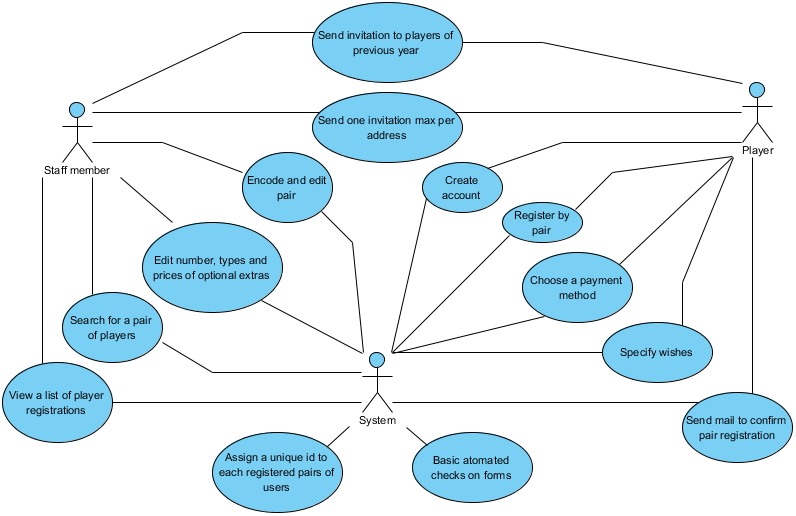
\includegraphics[scale=0.6]{PlayerRegistration}}


\subsection{Registration of a court}

Name : Register a court in the database. \newline
Identifier : UC02 \newline
Basics course of action : \newline
\\
\centerline{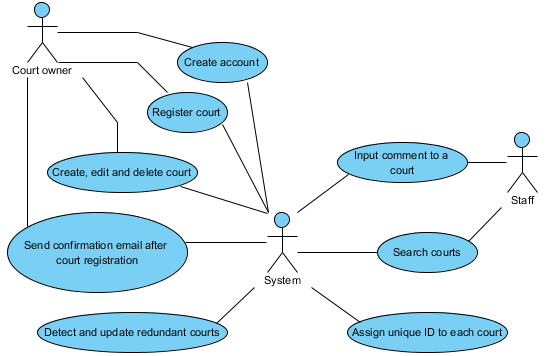
\includegraphics[scale=0.6]{CourtOwnerRegistration}}


\subsection{Creation of a group}

Name : Create a group of players. \newline
Identifier : UC03 \newline
Basics course of action : \newline
\centerline{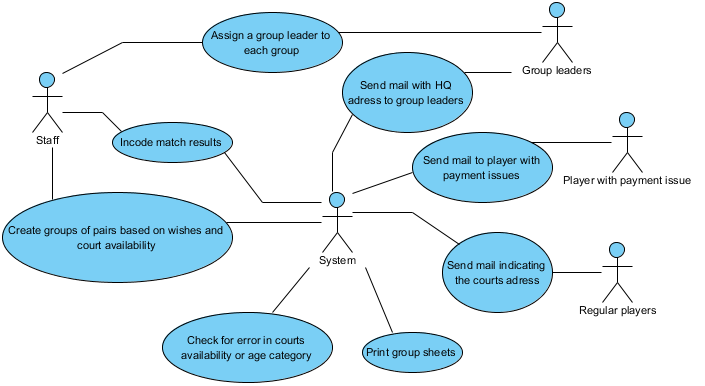
\includegraphics[scale=0.6]{GroupCreation}}

\subsection{Knock-off Tournament}

Name : Create a knock-off tournament. \newline
Identifier : UC04 \newline
Basics course of action : \newline
\centerline{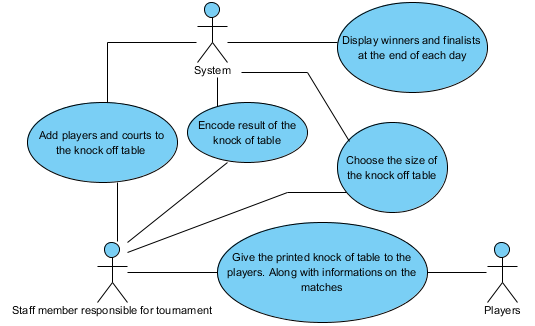
\includegraphics[scale=0.6]{KnockOffTournament}}

\subsection{Activity diagrams}
\todo[inline]{A faire pour le 25 septembre\ldots}
\section{Initial planning}
\todo[inline]{Cette partie est à refaire complètement : il faut indiquer
comment on a fait pour définir la charge de travail et dire ce qui sera
implémenté à chaque deadline.}
We met many times to start this project. However, we know that our
schedules don't permit that every week, we will have to meet only once a
week (on Wednesday). There we will share our ideas and problems ;
other tools like Trello and GitHub will also improve our vision about
progression of the project. However, part of the team will meet on an ad
hoc basis according to the tasks. Here is our first schedule based on
the Poker Planning : \newline

\noindent\begin{longtable}{|p{0.275\linewidth}|p{0.725\linewidth}|}
    \hline
    Date & Themes \\
    \hline
    \hline
    17/09/2015 (Thur) 10.45 & Paperwork reading, choice of a project
    manager \\
    \hline
    17/09/2015 (Thur) 14.00 & Requirements analysis (1/2) \\
    \hline
    18/09/2015 (Friday) 14.00 & Requirements analysis (2/2) \\
    \hline
    23/09/2015 (Wed) 11.00 & Meeting : Poker planning, diagrams,
    discussion about tools, initialization of backlog in Trello \\
    \hline
    25/09/2015 (Friday) & Deadlines for requirements, development methodology
    and planning \\
    \hline
    30/09/2015 (Wed) 11.00 & Meeting \\
    \hline
    07/10/2015 (Wed) 11.00 & Meeting \\
    \hline
    09/10/2015 (Friday) & Deadline 1st iteration : wireframes, mockups \\
    \hline
    14/10/2015 (Wed) 11.00 & Meeting \\
    \hline
    21/10/2015 (Wed) 11.00 & Meeting \\
    \hline
    23/10/2015 (Friday) & Deadline 2nd iteration : all the must-have
    should be implemented with minor imperfection, see
    page~\pageref{musthave} \\
    \hline
    28/10/2015 (Wed) 11.00 & Meeting \\
    \hline
    30/10/2015 (Friday) & Deadline for the report on the teamwork \\
    \hline
    04/11/2015 (Wed) 11.00 & Meeting \\
    \hline
    11/11/2015 (Wed) 11.00 & Meeting \\
    \hline
    13/11/2015 (Friday) & Deadline 3rd iteration : Link to deployed
    application with mandatory requirements + should have requirement,
    see page~\pageref{shouldhave}\\
    \hline
    18/11/2015 (Wed) 11.00 & Meeting \\
    \hline
    25/11/2015 (Wed) 11.00 & Meeting \\
    \hline
    27/11/2015 (Friday) & Deadline 4th iteration : Implementation (almost)
    finished \\
    \hline
    02/12/2015 (Wed) 11.00 & Meeting \\
    \hline
    09/12/2015 (Wed) 11.00 & Meeting \\
    \hline
    15/12/2015 (Tue) & Deadline for project defence, final product
    demonstration \\
    \hline
\end{longtable}

